\section{PreProject}
\subsection{Rich Picture}

\begin{figure}[h!]		%Remember to put the h!, to not fuck the sections.
 \begin{centering}
  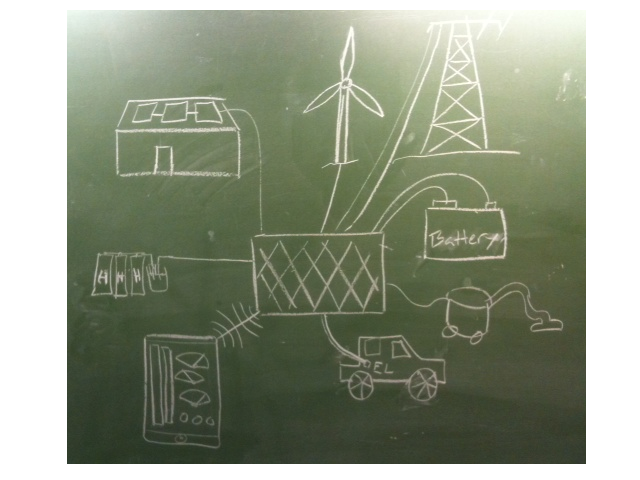
\includegraphics[width=1\textwidth]{images/rich_picture.png}
   \caption{The surrounding environment is shown in the rich picture. The
 			 elements are: solar-panels, hydrogen storrage, battery-charger, windturbine
 			 converter, userinterface, the electric grid and different loads such as a
 			 hyrogen engine, vacumcleaner etc. }
 \end{centering}
\end{figure}

\subsection{Storry Telling}
Aarhus University, a place full of innovation and great ideas. Jan Nielsen
welcomes a class of high-school students to the green system simulator. Here it
is possible to see how much energy you can get out of green energy harvesting
such as wind and solar energy. When the system produces to much energy, the 
energy is stored in form of Hydrogen. The Hydrogen is to be used for a Hydrogen
driven engine which is placed nearby the green system simulator. Here people can
really come an get an idea about how much they can help the environment, but
also their own wallet, if they invest in some green energy for their own house.
The guests can navigate around on a screen to see how much energy each device 
creates or consumes, this is shown in a down to earth way, where everybody can follow, 
even persons without no special education or courses in the energy field.
\subsection{Storycards}
\textbf{Story Card 1:} I want to be able see how much energy is being harvest by
the wind turbines and solar panels and how much energy is being consumed, this should be
a user friandly graphycal interface.\\\\
\textbf{Story Card 2:} When the energy production is higher (batteries full
charged, and no loads connected), the energy should be stored as hydrogen in a safe way so
later it can be converted again to energy by a fuel cell or used as gas for a
hydrogen car.\\\\
\textbf{Story Card 3:} In order to show of, the interface has too be userfriedly
and easy too use, so students coming over to AU - Herning without any energy
knowledge should be able to easly navigate the system.\\\\
\textbf{Story Card 4:} The system will be in a outside enviroment, so it as to
be robust against weather conditions and people temper.\\\\
\textbf{Story Card 5:} When batteries and hydrogen tanks are fully charged, the
energy should be provided in to the national power grid or/and university electrical
system.\\\\
\textbf{Story Card 6:} For further improvements and development the system have
to be fully documented, scalable and modular hardware construction.\\\\

\subsection{Preliminary Use Cases}

\subsection{Stakeholder Analysis}
Who is responsible for what ?\\
Morten + Klaus: Project coordinators (something like that)\\
Per - He got the money\\
Jan - Our customer\\
2. Customer that should specify layout of homepage (probably an e09 student)\\
Kristian, Henning ? Any more Biatches ?


\begin{figure}[h!]
 \begin{centering}
  \begin{tabular}{| l | l | l | }
   \hline
      & Has decision power & Has no decision power \\ \hline
    Directly involved stakeholder & 5 & Klaus Kolle Morten Opprud \\ \hline
    Not directly involved stakeholder & 10 & 9 \\
    \hline
   \end{tabular}
  \end{centering}
 \caption{Stakeholder table}
\end{figure}

\subsection{System Definition}
\textbf{Proposal 1:}\\	
When devices is connected to the Energy HUB, it automatically sees if is a input
or an output device.
\\\textbf{Proposal 2:}\\
Something to proposal 2.\\
